The LHC is a $pp$ collider, located at Geneva, Switzerland.
% Talk about the LHC being a hadron collider and the difficulties associated
% with it
Unlike electrons and positrons, the proton is a composite particle made of
$u, u, d$ quarks as well as other virtual partons.
All these particles participate in the $pp$ collision, carrying
varying portion of the total momentum.
The exact fraction of momentum carried by each type of parton is described by
parton distribution function\footnote{
    The parton distribution function is defined as:
    Number density to find fraction of the momentum (denoted as $x$) at certain
    squared energy scale $Q^2$.
} \cite{Ball:2014uwa}.
Since the precise fraction of momentum carried by interacting
partons\footnote{
    Again, these are characterized by parton distribution functions
} is unknown, the $B$ meson rest frame is not readily calculable.

Because many partons, such as quarks and gluons, can interact both
electroweakly and strongly,
the cross section of $b \bar{b}$ is larger than that of the $B$ factories, as a
result, more $b \bar{b}$ events are generated.
The measured $b \bar{b}$ cross section at LHCb in \SI{13}{TeV} $pp$
collisions\footnote{
    For $2 < \eta < 5$ only, since this is the LHCb acceptance range.
} is $144 \pm 1 \pm 21$~\si{\mu b} \cite{Aaij:2016avz}, whereas at the $B$
factories it is only about $1.05$~\si{nb} \cite{Harrison:1998yr}.
At the same time, unwanted particles will be generated frequently at hadron
colliders, leading to higher background.


% Talk about subdetectors
LHCb, a single-arm spectrometer, is one of the four large experiments at the
LHC.
Its constituent subdetectors, from closest to farthest from the collision point,
are shown in \autoref{fig:lhcb_detector_view}:
The Vertex Locator (VELO) provides precise measurements of track coordinates
close to the collision point.
Two Ring Imaging Cerencov counters (RICH1, RICH2) provide particle
identification for charged particles over a wide range of momentum.
The Tracker Turicensis (TT), Inner Tracker (IT), and Outer Tracker (OT) provide
additional tracking for charged particles and measure their momenta.
The calorimeters (ECAL and HCAL) have a first-level (L0) trigger to select
hadron, electron, and photon candidates based on their transverse momentum
$p_T$;
they also provide identification for the particles listed above;
finally, they provide energy and position measurements for these particles.
The Muon system (M1-5) is farthest from the collision point;
it provides L0 high $p_T$ muon trigger, and a high-level trigger (HLT) for muon
identification. Compared to the $B$ factories, LHCb trigger is not
inclusive---The trigger only selects specific decays \cite{LHCb:2008}.

\begin{figure}[ht]
    \centering
    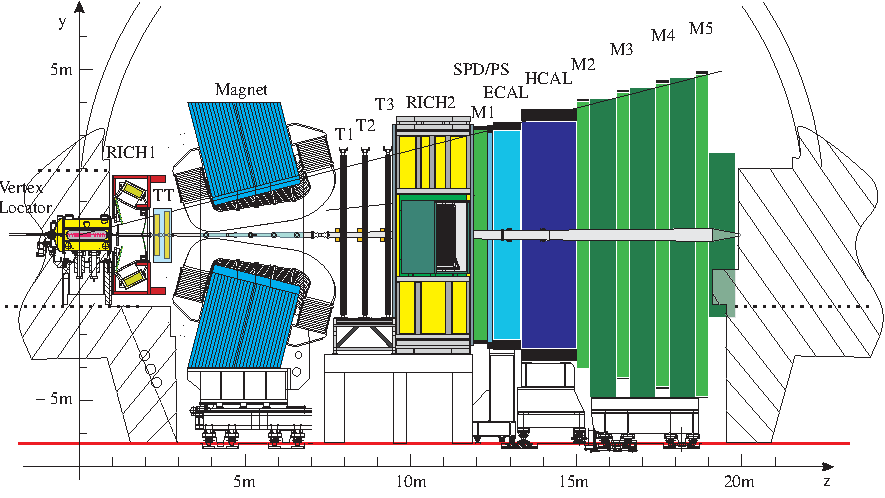
\includegraphics[width=0.7\textwidth]{figs/lhcb_detector_view.pdf}
    \caption{
        View of the LHCb detector and its subsystems.
        Extracted from \cite{LHCb:2003ab}.
    }
    \label{fig:lhcb_detector_view}
\end{figure}

% Talk about LHCb being forward-only
An interesting design choice is the geometry of the LHCb detector:
Instead of being a barrel $4\pi$ detector, it is forward-only.
This is because at high energies, $b\bar{b}$ is mostly produced in the forward
and backward direction.
The LHCb design is a cost-effective way to construct a detector at the LHC
dedicated for $B$ physics.

% Talk about tracking
LHCb has a very good vertexing and tracking system, achieving vertex resolutions
down to \SI{20}{\mu m} in a challenging environment.
However, due to the amount of material before the calorimeters and their poor
granularity,
reconstruction of neutral particles, such as $\pi_0$, is less
precise \cite{LHCb:2008,Guz:2017}.
This is why LHCb analyses typically focus on final states with charged particles
only, whereas $B$ factories can afford to use final states with neutral
particles.

% Talk about run 1 and run 2 luminosity
LHCb collected data from 2010 to 2012 with a center of mass energy of
\SI{8}{TeV}, and from 2015 to 2018 at \SI{13}{TeV}.
The total integrated luminosity during these two periods is about
\SI{9.2}{fb^{-1}} \cite{LHCb-Lumi:2019}.
% Talk about LS2 upgrade and LHCb's future
Currently, LHCb is shut down for an upgrade which will greatly increase the
readout rate of the detector starting in 2021.
